\chapter{Image recognition algorithms}
\label{algorithms}
This chapter presents several techniques for~object detection in an image. In~the first \mbox{section}~\ref{algorithms-classical} are introduced two representatives of~classical computer vision algorithms. The~second section~\ref{algorithms-nn} focuses on~the neural network approach. Not all of~the described algorithms are used in~the final solution, however, all of~them are at~least options and provide context for~the selected ones.

\section{Classical computer vision techniques}
\label{algorithms-classical}
While using classical computer vision algorithms might seem irrelevant in~the era of~neural networks, it is not entirely so. They do not require any training and the computation is very fast. Moreover, keyboards are usually quite contrastive (dark text on~a light background and vice versa) which presents opportunities for~detectors based on edges or colors.

\subsection{Canny edge detector}
\label{algorithms-classical-canny}
This detector was developed by~John Francis Canny in~1986. Since~the original paper~\cite{canny-paper}, the algorithm has undergone slight modifications. Currently, one of~the most used implementations is the one from~OpenCV library~\cite{opencv-library}, which consists of~several steps:

\begin{enumerate}[topsep=0pt,itemsep=-1.5pt,partopsep=6pt]
  \item \emph{Noise reduction}\\
  Edge detection is very susceptible to~noise. For that reason, the image is blurred by~a Gaussian filter. As a consequence, the true edges will stand out.
  \item \emph{Gradient calculation}\\
  The Sobel filter is applied to~the image to~obtain horizontal and vertical derivatives~\ref{canny-sobel}.
  \begin{equation}
  \label{canny-sobel}
  G_x = \begin{bmatrix}
            1 & 0 & -1\\
            2 & 0 & -2\\
            1 & 0 & -1
        \end{bmatrix} * image, \quad
  G_y = \begin{bmatrix}
            1 & 2 & 1\\
            0 & 0 & 0\\
            1 & 2 & 1
        \end{bmatrix} * image
  \end{equation}
  The magnitude~\ref{canny-gradient-magnitude} and angle~\ref{canny-gradient-angle} of~the directional gradients can be computed as follows:
  \begin{equation}
  \label{canny-gradient-magnitude}
  |G| = \sqrt{G_x^2 + G_y^2}
  \end{equation}
  \begin{equation}
  \label{canny-gradient-angle}
  Angle(G) = arctan(G_x^2/G_y^2)
  \end{equation}
  \item \emph{Non-maximum suppression}\\
  This stage tests each pixel for~being a local extreme in~the direction of~the gradient. If~not, it is suppressed.
  \item \emph{Hysteresis thresholding}\\
  The detector accepts 2~parameters, high and low thresholds. Edges with~an intensity gradient higher than the upper threshold are considered \say{sure edges} and are accepted by~the algorithm. On~the other hand, edges with~gradients lower than the lower threshold are suppressed. Edges with gradients in~between are kept only if they are connected to~a \say{sure-edge}.
\end{enumerate}

The result of~the algorithm is a binary image. Bounding boxes can be constructed by~computing contours. The following images~\ref{algorithms-canny-binary},~\ref{algorithms-canny-binary-bboxes},~\ref{algorithms-canny-result-bboxes} demonstrate the keyboard keys detection using the canny detector.
\begin{figure}[hbt]
    \centering
    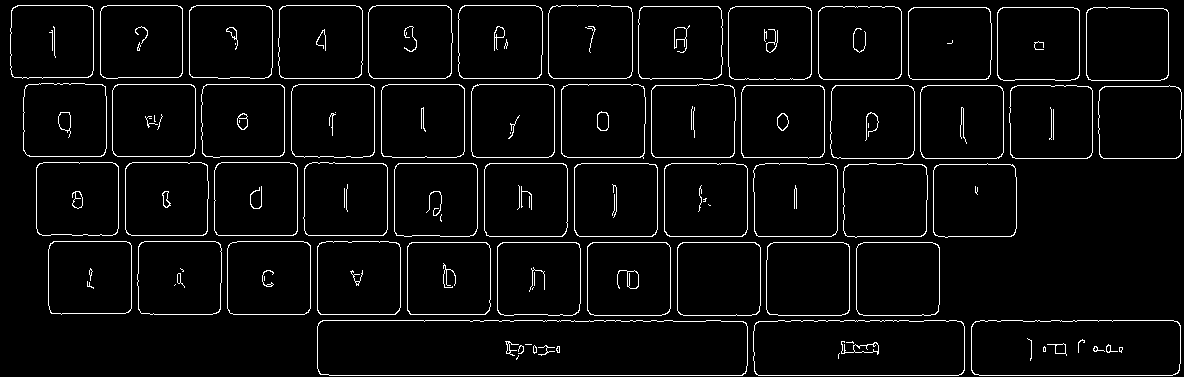
\includegraphics[width=1\textwidth]{img/algorithms/canny-binary.png}
    \vspace{-15pt}
    \caption{Canny detector creates a binary image with discovered edges.}
    \label{algorithms-canny-binary}
\end{figure}

\begin{figure}[hbt]
    \vspace{-9pt}
    \centering
    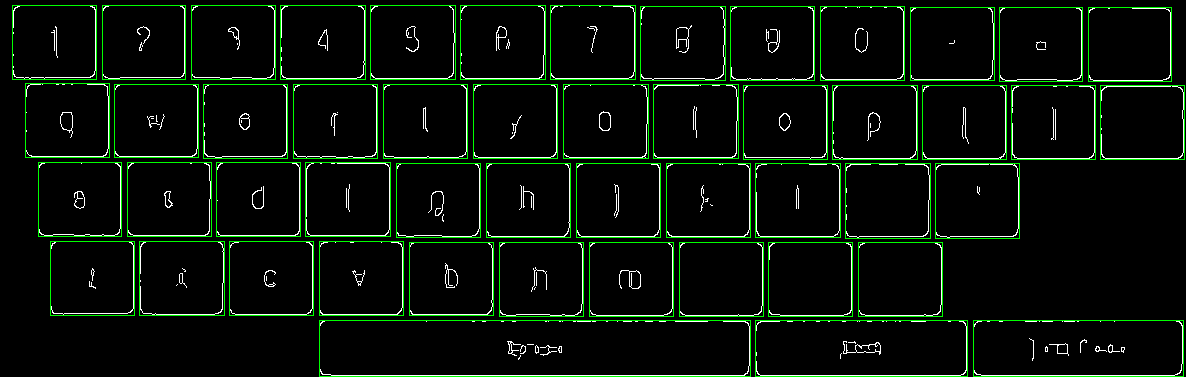
\includegraphics[width=1\textwidth]{img/algorithms/canny-binary-bboxes.png}
    \vspace{-15pt}
    \caption{Contours and their bounding boxes can be computed from the binary image.}
    \label{algorithms-canny-binary-bboxes}
\end{figure}

\begin{figure}[hbt]
    \vspace{-9pt}
    \centering
    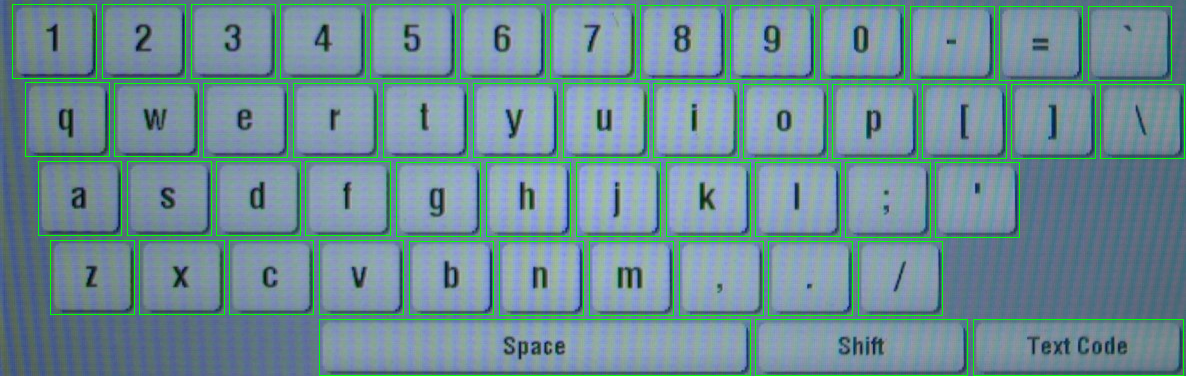
\includegraphics[width=1\textwidth]{img/algorithms/canny-result-bboxes.png}
    \vspace{-15pt}
    \caption{Canny algorithm is capable of detecting key regions on a keyboard.}
    \label{algorithms-canny-result-bboxes}
\end{figure}

\subsection{Thresholding}
\label{algorithms-classical-thresholding}
Thresholding is a method which converts a polychromatic image to a binary one (\hbox{usually} black-and-white). To obtain pixel intensities, the image is typically converted to~grayscale representation. Then a~\hbox{threshold} is chosen and pixels with~intensities above this \hbox{threshold} are set to~one value (white) and the ones below to~another (black). The computation is described by~formula~\ref{thresholding-binary-formula}, where \(I(x, y)\) is pixel intensity on~position \([x, y]\), \(T\) is a threshold and \(G(x, y)\) is the resulting pixel value.

\begin{equation}
  \label{thresholding-binary-formula}
  G(x, y) = \begin{dcases}
 255 & \text{if}\hspace{6pt}I(x, y)\ge\text{T}
 \\
 0 & \text{else}
 \end{dcases}
\end{equation}

However, this method is quite trivial and doesn't work well with~images with different light conditions~\cite{opencv-library}. In~such cases, a different approach such~as adaptive thresholding should be used which computes the threshold from~the neighborhood of~the given pixel. Figure~\ref{algorithms-thresholding-local-global} shows the different results from~global and local thresholding.

\begin{figure}[hbt]
	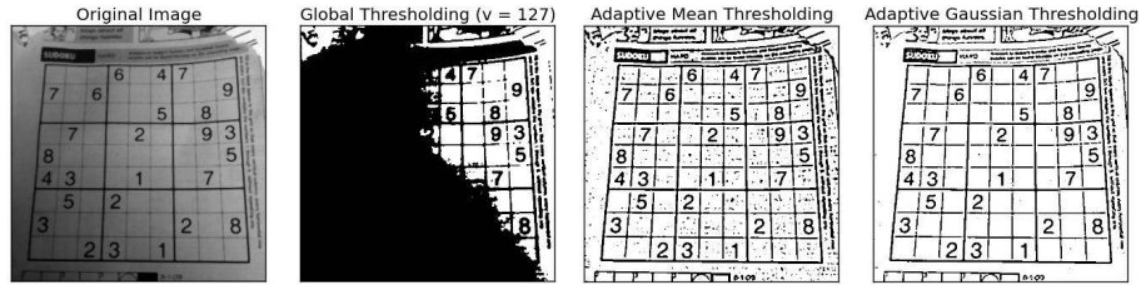
\includegraphics[width=1\textwidth]{img/algorithms/thresholding-local-global.png}
	\caption{Difference between global and adaptive local thresholding (adapted from \cite{opencv-library})}
	\label{algorithms-thresholding-local-global}
\end{figure}

Another popular thresholding method is Otsu's binarization. It is effective and does not require a threshold specification. This method computes probabilities of~pixel intensity values and constructs a histogram. The histogram usually contains~2 major peaks (classes), which represent background and foreground~\cite{opencv-library}. By~iterating over all possible threshold values within the intensity range, the algorithm selects a threshold with~minimum \hbox{intra-class} variance~\cite{otsu-binarization}. Following figure~\ref{algorithms-thresholding-otsu} depicts a~result of~Otsu's thresholding.

\begin{figure}[hbt]
	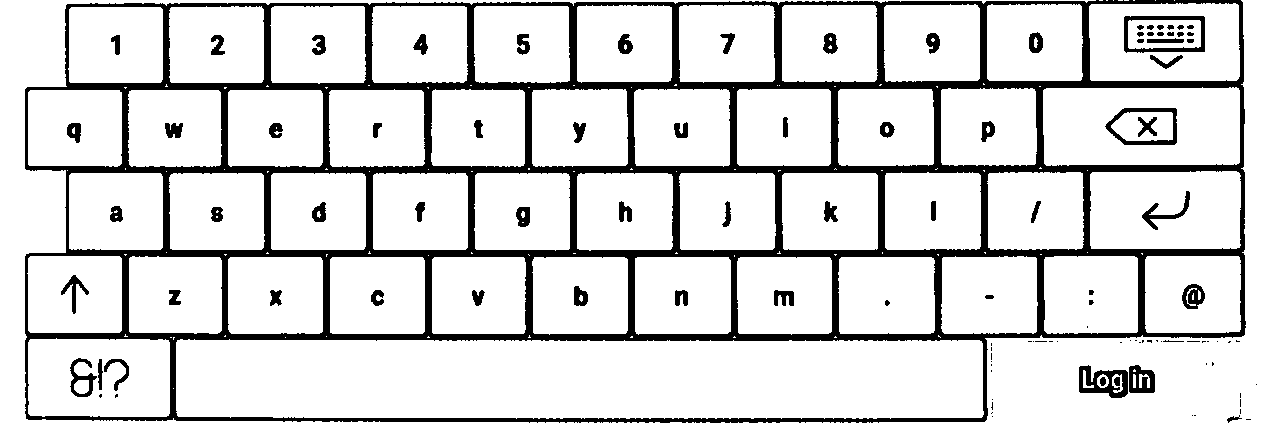
\includegraphics[width=1\textwidth]{img/algorithms/thresholding-otsu.png}
	\caption{Keyboard keys can be detected using Otsu's binarization and bounding boxes acquired by contours computation same as in Canny detector approach \ref{algorithms-classical-canny}.}
	\label{algorithms-thresholding-otsu}
\end{figure}

\section{Neural networks}
\label{algorithms-nn}
Since the success of~AlexNet in~the ILSVRC competition in~2012, convolutional neural networks have become the backbone of~computer vision. There exist many sub-domains of computer vision such as classification, segmentation or image restoration and new ones emerge every day. This section takes a closer look at~object detection sub-domain. The~main problem in~object detection is the localization of the target objects. The objects can be anywhere and by~using classification, a sliding window would have to be used which would classify the object in~it or not. The issue with~this approach is the variability in~the size of~the objects and the number of~classifications necessary. Therefore, new algorithms had to be devised and the next sections describe the most iconic ones.

\subsection{R-CNN}
\label{algorithms-nn-rcnn}
To solve the issue of~a large amount of~sliding window positions for~classification, R-CNN selects only~2000 region proposals using Selective Search algorithm~\cite{selective-search} which can be summed up~to~3 phases~\cite{r-cnn-medium}:

\begin{enumerate}[topsep=0pt,itemsep=-1.5pt,partopsep=6pt]
    \item Generate candidate regions using segmentation.
    \item Merge similar regions using a greedy algorithm.
    \item Create final region proposals.
\end{enumerate}

Once the regions are obtained, each of~them goes into~a ConvNet~\cite{r-cnn-cnn} which extracts \hbox{a 4096-long} feature vector~\cite{r-cnn}. This vector is then classified by the SVM~\cite{svm} algorithm. Apart from the actual detection, 4~offset values are predicted to~improve the bounding box precision (e.g.~part of~the object may be cut, so to~correct it)~\cite{stanford-object-detection-lecture}. Figure~\ref{algorithms-rcnn} demonstrates the whole detection process.

\begin{figure}[hbt]
    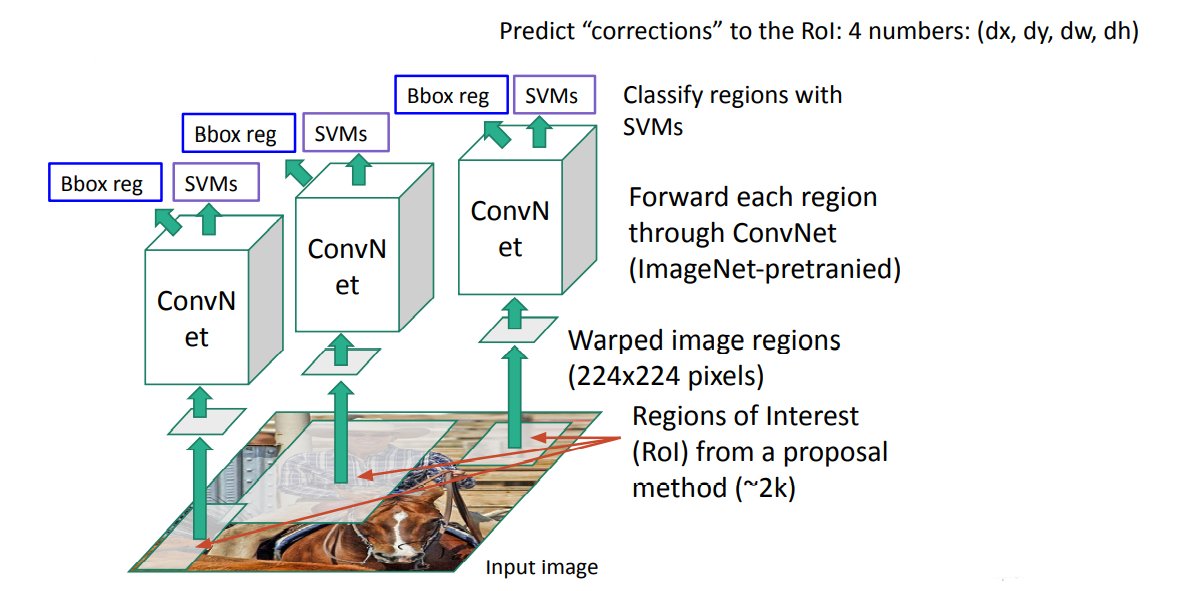
\includegraphics[width=1\textwidth]{img/algorithms/rcnn.png}
    \caption{Object detection process used by R-CNN (adapted from~\cite{stanford-object-detection-lecture})}
    \label{algorithms-rcnn}
\end{figure}

R-CNN achieved remarkable accuracy for~its time and significantly contributed to~the development of~specialized architectures for~object detection. For~instance, on~PASCAL VOC~2012 it improved the accuracy by~30~\% in~comparison to~the best previous result~\cite{r-cnn}.

\subsection{Fast R-CNN}
\label{algorithms-nn-fast-rcnn}
In~spite of~great object detection accuracy, R-CNN is very slow and computationally \hbox{expensive}. Therefore, the author of~the R-CNN tackles the drawbacks in~a new paper~\cite{fast-rcnn}. There are several issues he wanted to~solve:

\begin{enumerate}[topsep=0pt,itemsep=-1.5pt,partopsep=6pt]
    \item \emph{Multi-stage pipeline training} - ConvNet, SVM and bounding box regressors are trained separately.
    \item \emph{Expensive training} - It takes time to~classify~2000 region proposals per~image and space to~store features for~each of~them for~both SVM and bounding box regressors.
    \item \emph{Slow detection} - Features must be extracted for~each region proposal, which means running ConvNet forward pass, and there is no computation sharing.
\end{enumerate}

To~improve the detection speed, features are no longer extracted from~the regions, but instead, the whole image is processed by~the ConvNet. By~doing that, the feature extraction is run only once and the whole image feature map is obtained. An~ROI pooling layer is then used to create a feature vector for~each region proposal. ROI is a window of~rectangular shape which is divided into sub-windows and standard max-pooling is performed on~each of~them~\cite{fast-rcnn}. It is based on~the spatial pyramid pooling layer in~SPPnets~\cite{sppnet} and the same size output is ensured for~the subsequent fully-connected layers as~is depicted in~figure~\ref{algorithms-fast-rcnn-roi}. After~that, the softmax loss function is used to~predict the object class and a bounding box regressor the offset. Due to~2~output layers and single-stage training goal, a multi-task loss is introduced which combines both layers' losses and hence classification and bounding box regression can be trained together~\cite{fast-rcnn}. Full Fast R-CNN architecture is shown in~figure~\ref{algorithms-fast-rcnn}.

\begin{figure}[hbt]
    \centering
    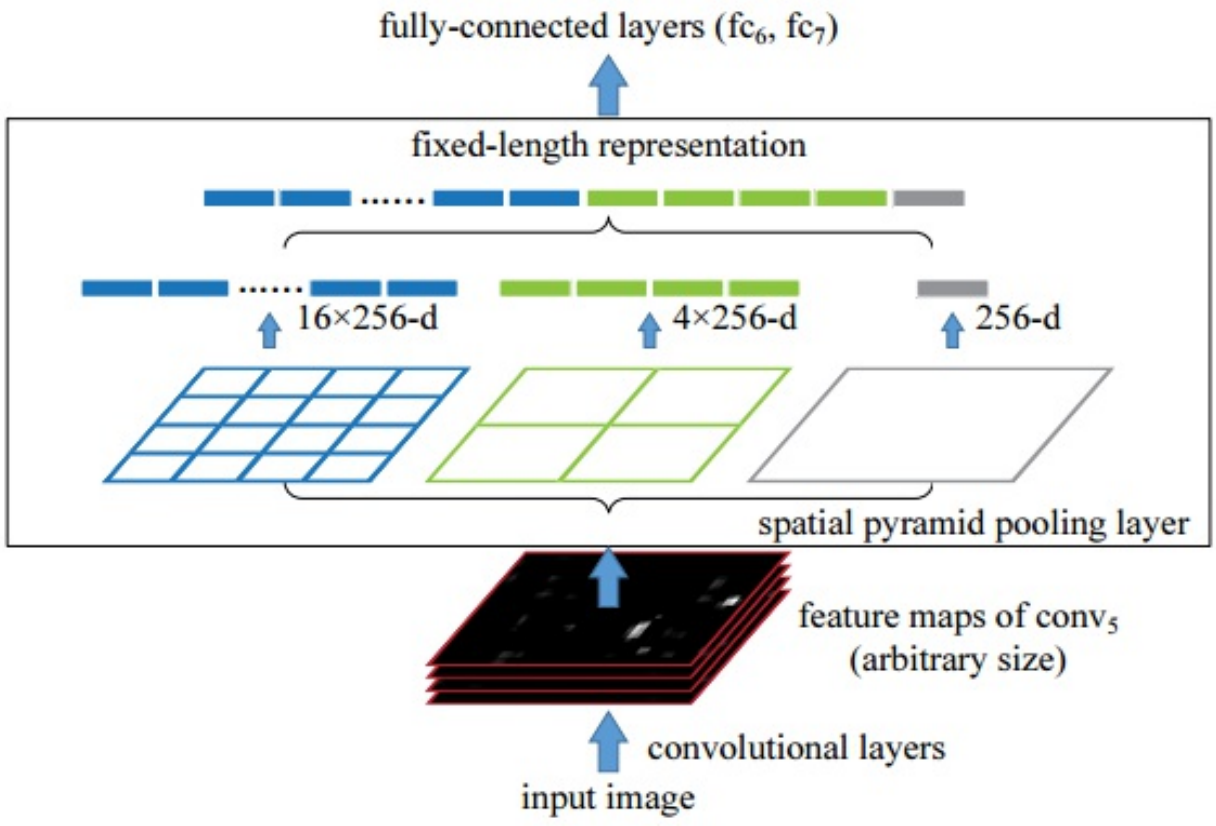
\includegraphics[width=0.8\textwidth]{img/algorithms/fast-rcnn-roi.png}
    \caption{ROI pooling layer in Fast R-CNN (taken from~\cite{hands-on-cnn})}
    \label{algorithms-fast-rcnn-roi}
\end{figure}

\begin{figure}[hbt]
    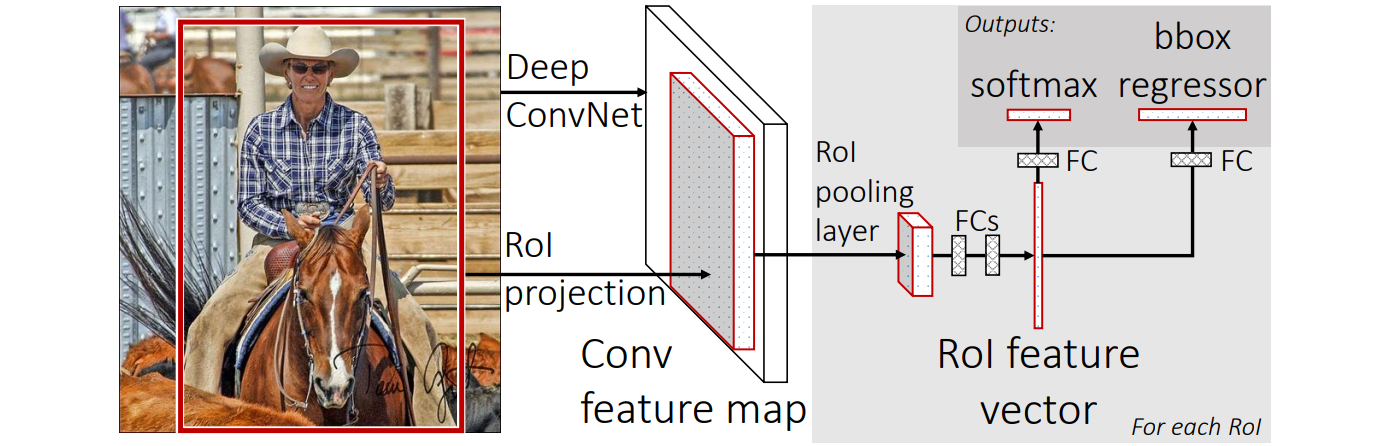
\includegraphics[width=1\textwidth]{img/algorithms/fast-rcnn.png}
    \caption{In Fast R-CNN, a feature map is extracted from~the input image and converted to~a feature vector by~the ROI layer. The softmax then makes the classification and the bounding box regressor finds the offset (taken from~\cite{fast-rcnn}).}
    \label{algorithms-fast-rcnn}
\end{figure}

Fast R-CNN managed to~fix all of the pin-pointed drawbacks. The training became single-stage which can update all layers at~once and there is no need to~store features on~disk anymore~\cite{fast-rcnn}. In~addition, detection is much faster and even more accurate~\cite{fast-rcnn}. Compared to~the R-CNN, training time got reduced almost 10 times and test time 23~times including the region proposals and nearly 147 times excluding them~\cite{stanford-object-detection-lecture}.

\subsection{Faster R-CNN}
\label{algorithms-nn-faster-rcnn}
R-CNN and Fast R-CNN share a common problem which is the use of~Selective Search algorithm for~region proposals. Selective Search on~its own is rather popular and effective, but in~comparison with~neural networks, it is slower by~a~margin as it takes around~2~seconds per~image to~find the regions~\cite{faster-rcnn}. It doesn't matter much to~R-CNN since it is quite slow and the performance hit is not so noticeable. However, Fast~R-CNN without the region proposals achieves almost real-time rates and the 2-second hit increases computation 7~times~\cite{stanford-object-detection-lecture}. Faster~R-CNN aims at replacing Selective Search with Region Proposal Network (RPN) as~shown in~figure~\ref{algorithms-faster-rcnn}.

\begin{figure}[hbt]
    \centering
    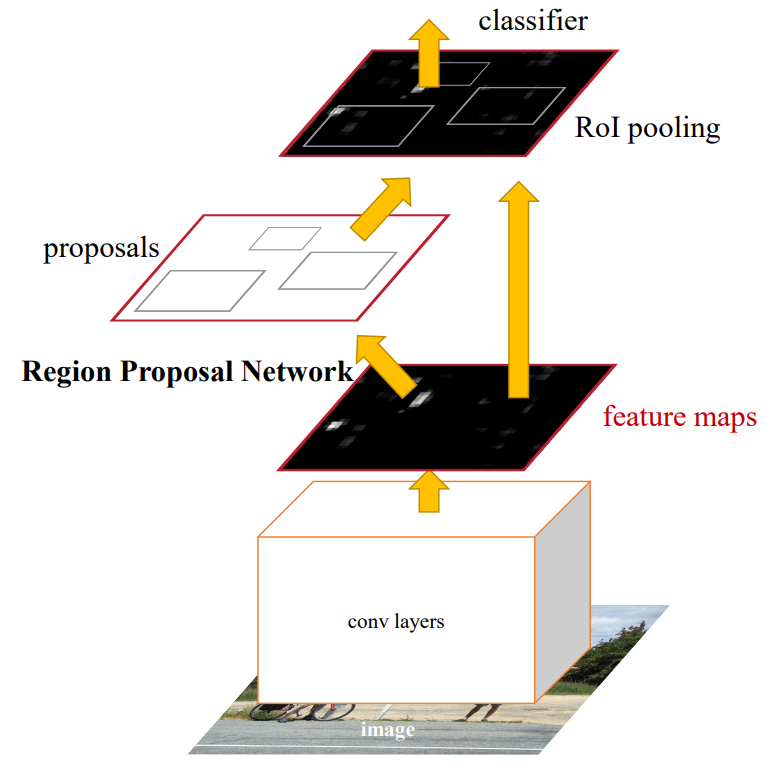
\includegraphics[width=0.6\textwidth]{img/algorithms/faster-rcnn.png}
    \caption{Faster R-CNN is essentially Fast R-CNN with~a neural network in~place of Selective Search (taken from~\cite{faster-rcnn}).}
    \label{algorithms-faster-rcnn}
\end{figure}

To understand better how RPN works and how it is included in~the model architecture, the \hbox{original} paper~\cite{faster-rcnn} describes it quite clearly. Still, I will provide a short summary. As~the idea is to train the whole model together, RPN shares the convolutional layers with the \hbox{Fast R-CNN} and works on~the output of~the last convolutional layer, the feature map. It~passes a \hbox{rectangular} sliding window through the map and generates several region proposals for~each window. The proposals are then parameterized relative to reference boxes called anchors. The anchors lie at~the center of~the sliding window and have different scales, so~the detection is \hbox{size-indifferent}. A~feature vector is extracted for~each proposal and a sibling \hbox{two-layer} network predicts the region coordinates and an objectness score defining, how sure it is that an object is in~the region. This is visualised in~figure~\ref{algorithms-faster-rcnn-rpn}.

\begin{figure}[hbt]
    \centering
    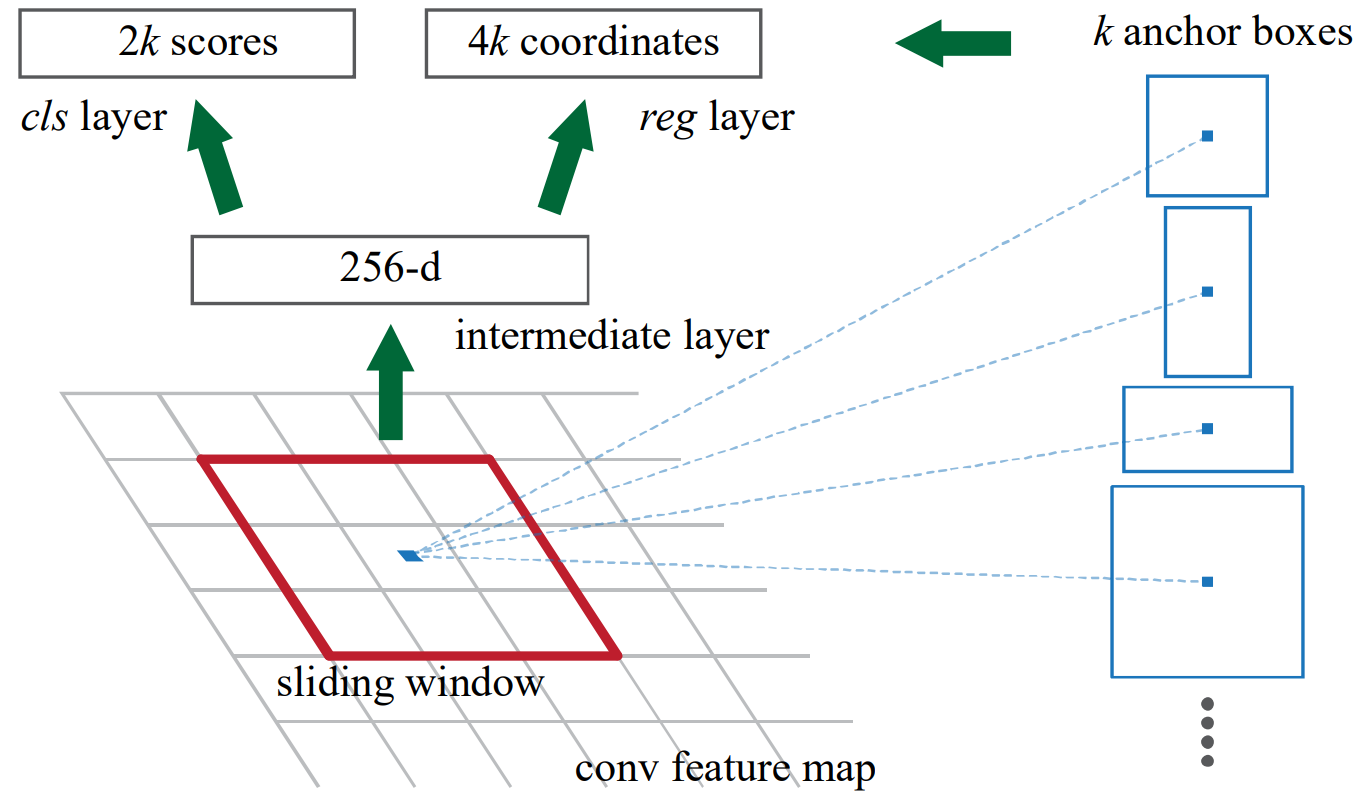
\includegraphics[width=0.7\textwidth]{img/algorithms/faster-rcnn-rpn.png}
    \caption{Region extraction in Region Proposal Network (taken from~\cite{faster-rcnn})}
    \label{algorithms-faster-rcnn-rpn}
\end{figure}

During the training, the intersection-over-union of~anchors and \hbox{ground-truth} boxes is computed. If an anchor is eighter the highest scoring or scores over~0.7~with any \hbox{ground-truth} box, it is assigned a positive label for~being an object. Having removed the Selection Search algorithm, it takes only~0.2 seconds to~process an image which makes it a real-time object detector and~11 times faster than the Fast R-CNN~\cite{stanford-object-detection-lecture}.

\subsection{YOLO}
\label{algorithms-nn-yolo}
YOLO (You only look once) brought a novel approach to~the object detection field. As~the authors of this algorithm~\cite{yolo} claim, the detection systems at~that time reused classifiers for the evaluation of certain windows in~an image. In~spite of~having methods for~selecting such windows, the R-CNN family is no different. What is more, the whole process is a pipeline of~several actions and all the R-CNN algorithms need to~look at~the image twice, once for~region proposal generation, and once for~object detection of~the proposals. YOLO, on~the other hand, needs only one look and is capable of~making the classification and bounding box regression simultaneously. Instead of~a single region, it sees the whole image which allows it to encode context information and as a result, it makes significantly fewer background errors than R-CNN based algorithms. Owing to all of~this, YOLO is extremely fast. Nevertheless, it lacked in~accuracy in~comparison with~the state-of-the-art approaches at~the time~\cite{yolo}.

The process of~finding the bounding boxes is described by~the paper~\cite{yolo} as~follows. The image is divided into a \(S\) x \(S\) grid which portrays figure~\ref{algorithms-yolo-grid} and a grid cell, which is a center of~an object, is responsible for~its detection. Each grid cell predicts \(B\) bounding boxes and their confidence scores, which reflects the intersection-over-uniou (IoU) with the ground-truth. To~predict a bounding box, the neural network uses features from the entire image. However, excess bounding boxes can be produced by neighboring grid cells for the same object. This is solved by non-maximal suppression. Apart from~the object location, the grid cell also predicts the object class probabilities.

\begin{figure}[hbt]
    \centering
    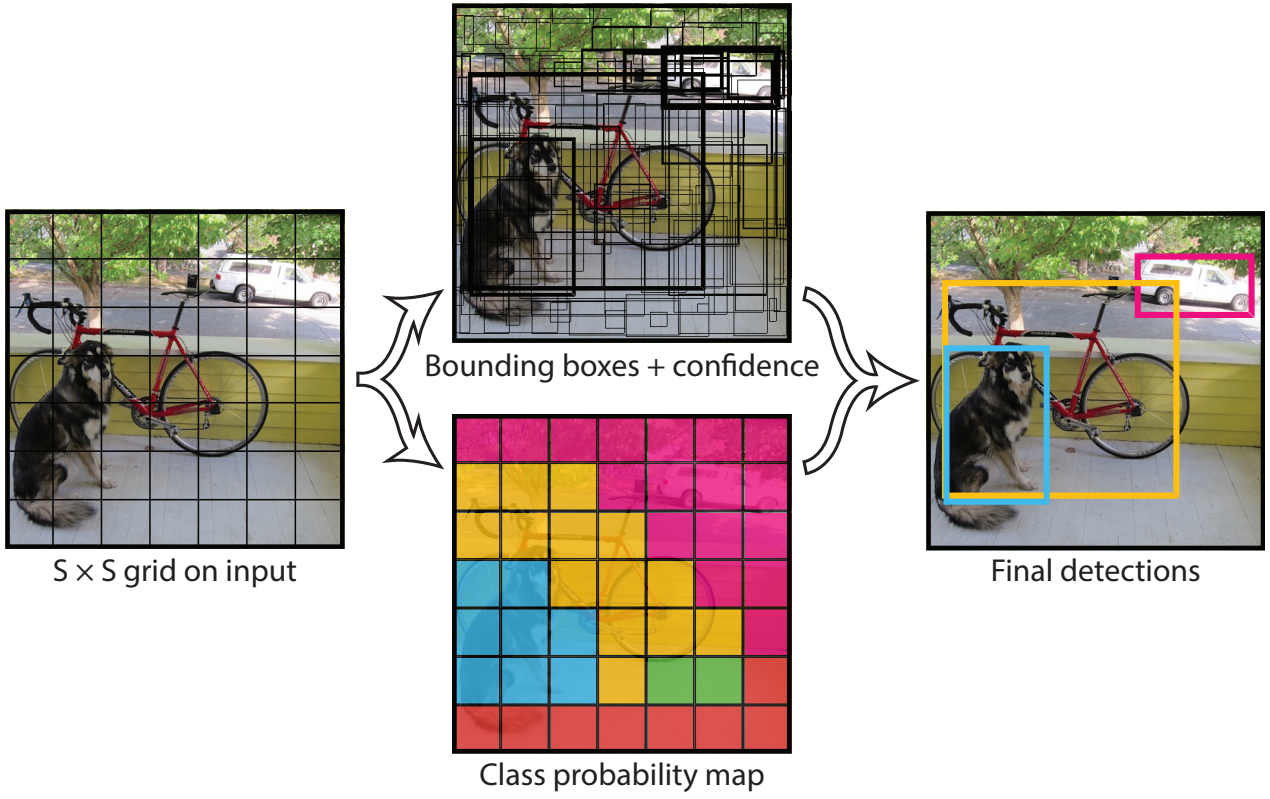
\includegraphics[width=0.9\textwidth]{img/algorithms/yolo-grid.png}
    \caption{YOLO uses a grid to~predict bounding boxes and object classes (taken from~\cite{yolo}).}
    \label{algorithms-yolo-grid}
\end{figure}

The architecture of~YOLO is based upon~the GoogLeNet~\cite{googlenet} with~the modification of~using 1x1 reduction layers followed by 3x3 convolutional layers instead of~GoogLeNet's inception modules~\cite{yolo}. Consequently, the network has~24 convolutional layers followed by~2~fully connected layers as~figure~\ref{algorithms-yolo-architecture} shows. The features are extracted by~the initial convolutional layers and the fully connected layers then produce the bounding boxes and class predictions~\cite{yolo}.

During the training, leaky ReLU activations are used in~the hidden layers and normal ReLU in~the final layer~\cite{yolo}. For~optimization, sum-squared error is utilized for~its simplicity, although it weights classification and localization errors equally, which is a downside~\cite{yolo}. The loss function is multi-part and consists of~5 terms. These terms are for~the object's center coordinates, bounding box dimensions, object class, a class in~case of~the object's absence and probabilities of~finding the same object respectively~\cite{yolo-evolution}.

\begin{figure}[hbt]
    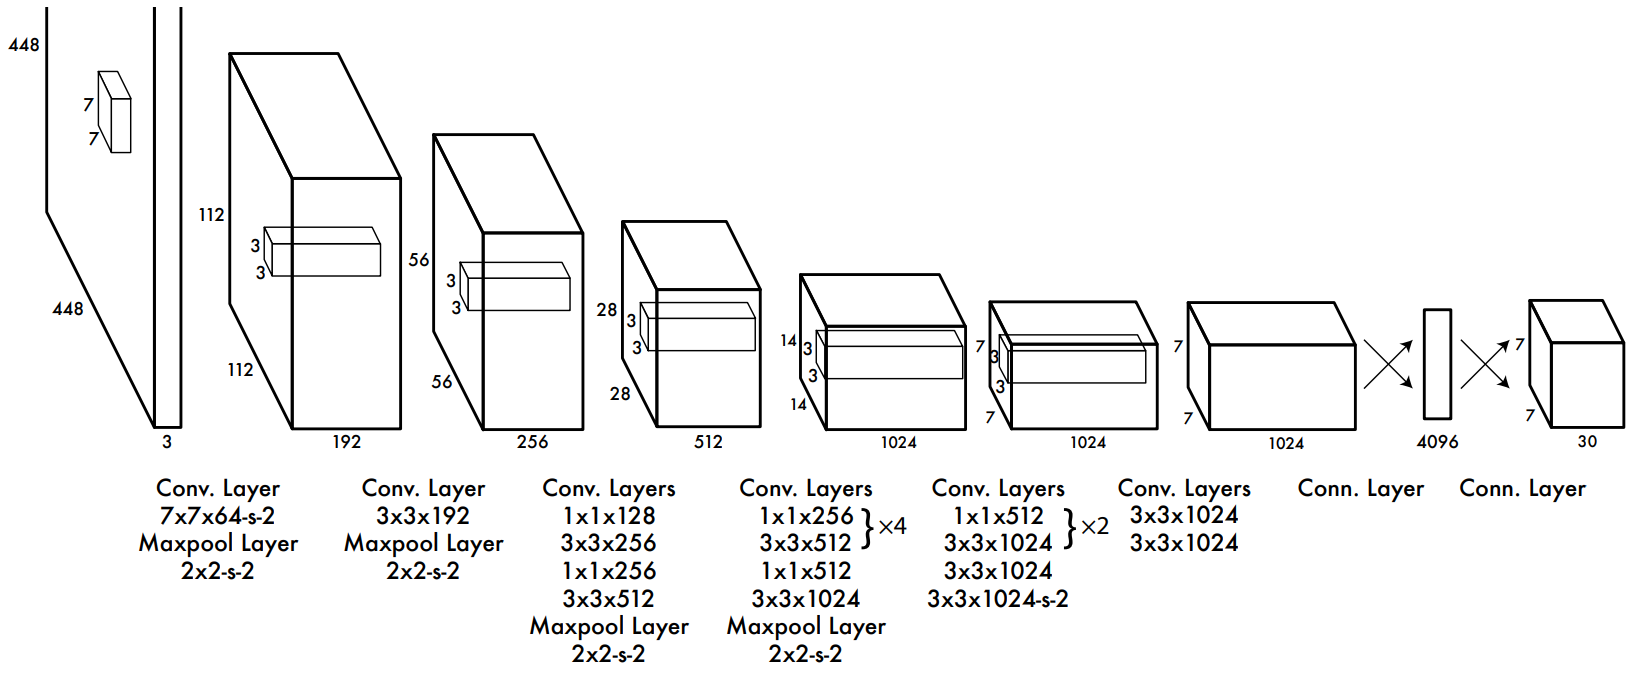
\includegraphics[width=1\textwidth]{img/algorithms/yolo-architecture.png}
    \caption{Architecture of YOLO network (taken from~\cite{yolo})}
    \label{algorithms-yolo-architecture}
\end{figure}

However, not even the novel approach of~YOLO is without limitations and the authors are well aware of them and mention them in the paper~\cite{yolo} as well. As each grid cell predicts only a few bounding boxes and a single class, it imposes a spatial constraint which causes difficulties in prediction of small objects like flocks of birds. Furthermore, it struggles with generalization of unusual aspect ratios. It has problems with localization errors. Still, it worked extremely well among other real-time object detectors and new versions fixing those issues have been being developed due to its popularity ever since.

\subsubsection{YOLOv2}

YOLOv2~\cite{yolov2} brought several improvements. These are very well summarized by~article~\cite{yolo-evolution} from~which the most important ones are listed:

\begin{itemize}[topsep=0pt,itemsep=-1.5pt,partopsep=6pt]
    \item Batch normalization is used instead of~dropout layers.
    \item Resolution detail is increased by the removal of~a max-pool layer, which leads to~better accuracy.
    \item Location is predicted with~respect to~a grid cell instead of~an anchor box. This means better stabilization during the training.
    \item Feature map is more fine-grained (13x13).
    \item Fully-connected layers are replaced with~convolutional ones, which allows for~multi-scale training.
    \item VGG-16 backbone is replaced by~Darknet-19.
    \item Hierarchical classification is introduced. This allows for~assigning several classes (e.g.~dog and their breed) to objects whereas before they were mutually exclusive.
\end{itemize}

As~a result, YOLOv2 improved especially in~accuracy, recognition of~smaller objects, but also in~speed. It became state-of-the-art in~both speed and accuracy without any obvious limitations.

\subsubsection{YOLOv3}
YOLOv3 focuses mainly on~improving speed and accuracy, rather than fixing some known issues as the name of~paper~\cite{yolov3} \say{YOLOv3: An Incremental Improvement} also suggests. This paper introduces the following changes. The objectness score is calculated using logistic regression and the sigmoid function is used to~predict the bounding box center. In~class prediction, a switch to~cross-entropy from~the sum-squared error was made. Moreover, a~new deeper backbone Darknet-53 is used.

\subsubsection{YOLOv4}
This version of YOLO is very important because the creator of~YOLO, Joseph Redmon, retired from~computer vision and new researchers continued with~YOLO advancements. They came to the conclusion, that a general object detector consists of~several parts, which are input, backbone, neck and head~\cite{yolov4}. They decided to map YOLO into this decomposition as~figure~\ref{yolov4-decomposition} depicts.

\begin{figure}[hbt]
    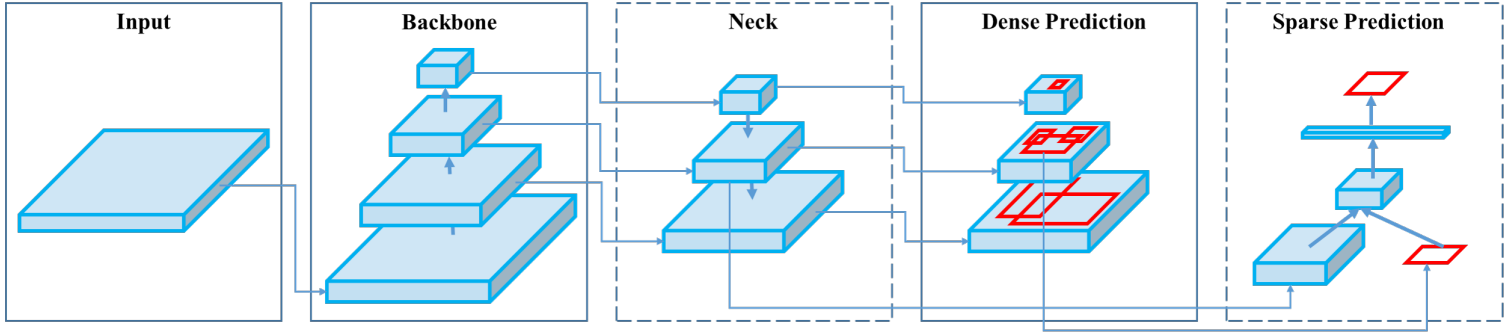
\includegraphics[width=1\textwidth]{img/algorithms/yolov4-decomposition.png}
    \caption{In~YOLOv4, input is the input image. Backbone is the feature extraction network which was updated from~Darknet53 in~YOLOv3 to~CSPDarknet53. The neck is supposed to~be the region selection part, the spatial pyramid pooling, which underwent subtle modification in~YOLOv4 to improve accuracy. Lastly, the head takes care of~the class and location prediction which in~this figure are the dense and sparse prediction blocks (adapted from~\cite{yolov4}).}
    \label{yolov4-decomposition}
\end{figure}

The new authors also introduce bag of~freebies and bag of~specials. Bag of~freebies are methods that improve performance without increasing inference time in~production~\cite{yolov4}. They can be viewed as some plugin modules which one can try to~improve a model. There is a huge amount of them and they are usually normalization or regularization methods, data augmentation, data imbalance etc. From~those that YOLOv4 uses can be named e.g.~Mosaic data augmentation, DropBlock regularization, class label smoothing and many othes~\cite{yolov4}. Concerning the bag of specials, those are post-processing methods which do have a small impact on~inference time but bring a significant accuracy increase. Out~of~these, mish activations, Cross-Stage Partial (CSP) Connection or SPP blocks for instance are applied in~YOLOv4~\cite{yolov4}.

\subsubsection{YOLOv5}
YOLOv5 was developed by~different authors than YOLOv4 and was released just a month after the previous version. Research on~both of~them started relatively at~the same time and was conducted simultaneously. It was named YOLOv5 simply to avoid a collision~\cite{yolo-evolution-thesis}. As~a result, due to the parallel work and application of~the same state-of-the art innovations in~the field, the architectures of~both do not differ much~\cite{yolo-evolution-thesis}. YOLOv4 paper even acknowledges Glenn Jocher, the author of YOLOv5, for~the Mosaic data augmentation~\cite{yolov4}. Consequently, both models perform very similarly, however, YOLOv5 appears to~be a bit faster and YOLOv4 slightly more accurate when more custom configuration is applied~\cite{yolov5-vs-yolov4}. Owing to the naming, timing, lack of~outstanding improvements in~comparison with~the previous version and most importantly no research paper, YOLOv5 was a source of~quite a controversy in~the computer vision community. Nevertheless, it got accepted eventually.

\subsubsection{YOLOv6}
YOLOv6 further advances both speed and accuracy of~YOLO algorithm and beats all other real-time detectors at~the time~\cite{yolov6}. It further improves the backbone which is now named EfficientRep consisting of~RepBlocks~\cite{yolov6}. These RepBlocks also replace the CSP blocks in~the neck~\cite{yolov6}. Main architectural change brings the head, though. Instead of~1~head,~3~heads are used as~figures~\ref{yolov6-architecture} and~\ref{yolov6-head} show.

\begin{figure}[hbt]
    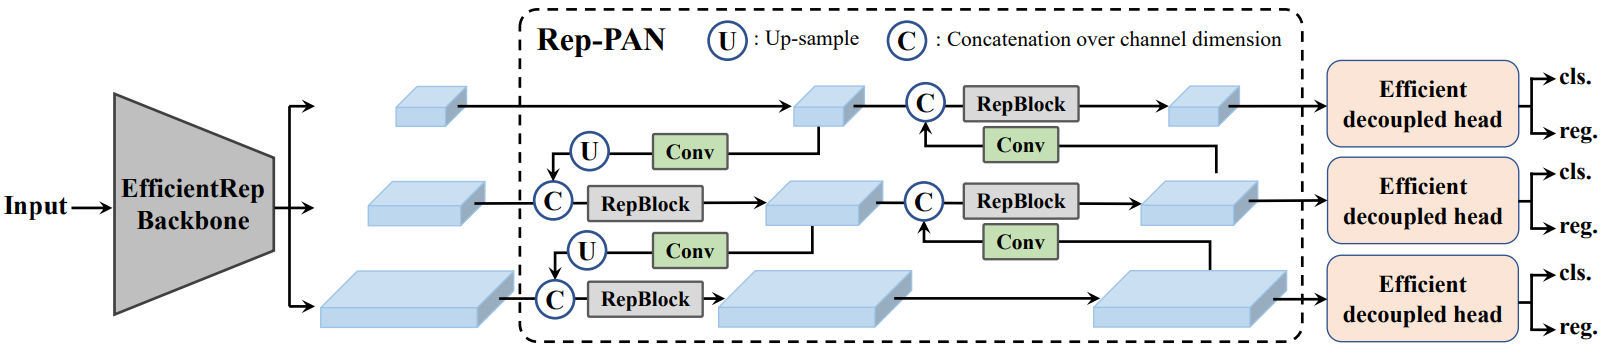
\includegraphics[width=1\textwidth]{img/algorithms/yolov6-architecture.png}
    \caption{In~YOLOv6, neck outputs go to~3 decoupled heads. In~the previous versions, localization and classification heads were coupled, which means that they shared the same features and more computation was needed~\cite{yolov6} (taken from~\cite{yolov6}).}
    \label{yolov6-architecture}
\end{figure}

\begin{figure}[hbt]
    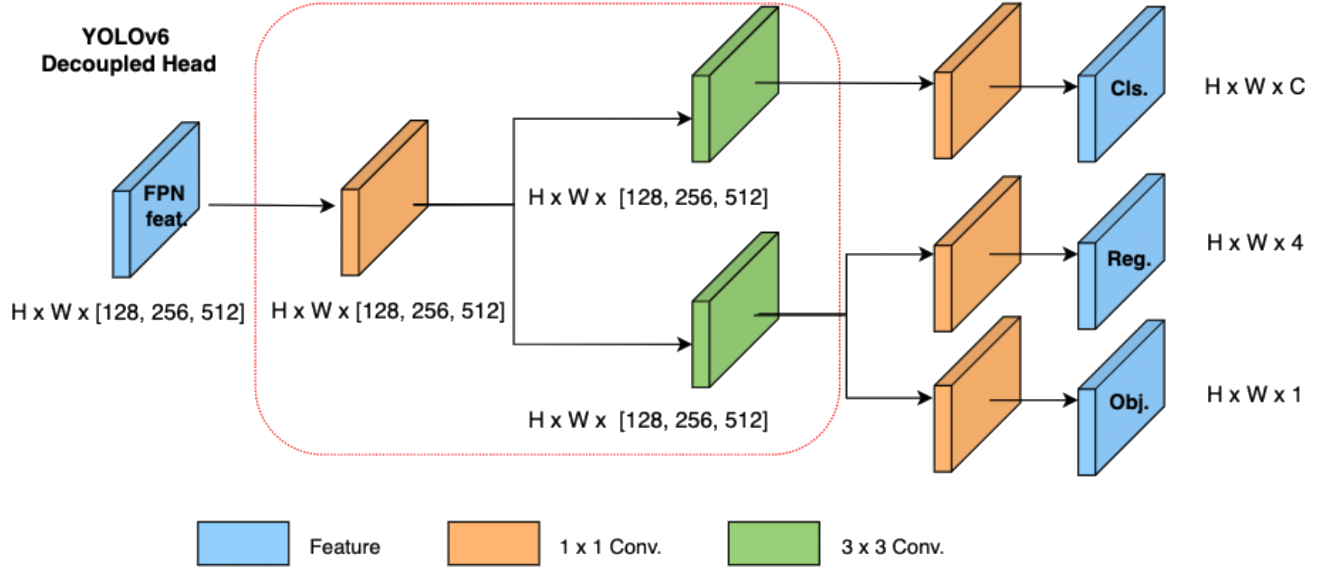
\includegraphics[width=1\textwidth]{img/algorithms/yolov6-head.png}
    \caption{In~a head, 3~loss functions are computed. Cross-entropy for classification and L1 for regression were left the same from~the previous versions. A~new object loss is \hbox{computed}, which aims at~reducing the score of~low-quality bounding boxes but unfortunately does not have many effects~\cite{yolov6} (taken from~\cite{yolov6-roboflow}).}
    \label{yolov6-head}
\end{figure}

\subsubsection{YOLOv7}
Similarly to~YOLOv4 and YOLOv5, the release of~YOLOv6 and YOLOv7 was very close. There are still debates about which one is better but more benchmarks found on~the internet favour the latter. Moreover, the YOLOv7 paper claims better results than YOLOv6 on~the COCO dataset~\cite{yolov7}. According to some~\cite{yolov7-web}, it is even expected of~YOLOv7 to~become the new industry standard. It might also be worth mentioning that YOLOv7 come from the same authors as~YOLOv4. The most important contributions of~YOLOv7 are the following:~\cite{yolov7}

\begin{itemize}[topsep=0pt,itemsep=-1.5pt,partopsep=6pt]
    \item \emph{Extended efficient layer aggregation} -- Efficiency of~the convolutional layers is the key to~the inference speed. Hence, building heavily on~research on~this topic, using group convolution to~increase feature cardinality and combining features of~different groups leads to an improved feature learning process.
    \item \emph{Model scaling for concatenation-based models} -- While other models usually scale the width or~depth of the network, YOLOv7 scales them together which keeps the architecture optimal for~different sizes.
    \item \emph{Planned re-parameterized convolution} -- Re-parameterization means averaging weights to~create a more robust model. Which network modules to~re-parameterize is determined by~gradient flow propagation paths.
    \item \emph{Auxiliary heads} -- Network heads making the prediction are quite far. Other heads placed in~the middle of~the network help with the training.
\end{itemize}

\subsubsection{Others}
Apart from the main versions of~YOLO, other YOLO mini-series such as~YOLOX, YOLOR or PP-YOLO have emerged. They (and their newer versions) usually build upon a~current YOLO version and improve it in~certain ways. YOLOX for example removes the anchor boxes and YOLOR combines explicit and implicit knowledge to~perform several tasks. However, covering all these YOLO offspring is out of~scope of~this thesis.

\subsection{Single Shot Detector}
\label{algorithms-nn-ssd}
Similarly to~YOLO, Single Shot Detector (SSD) needs only one look at~an image to process it. At~the time, it outperformed both YOLOv1 and R-CNN-based algorithms in~speed and accuracy alike~\cite{ssd-paper}. Same as~the original YOLO, it uses the VGG-16 net as~a backbone on~which it builds additional convolutional layers as~depicted in~figure~\ref{ssd-architecture}.

\begin{figure}[hbt]
    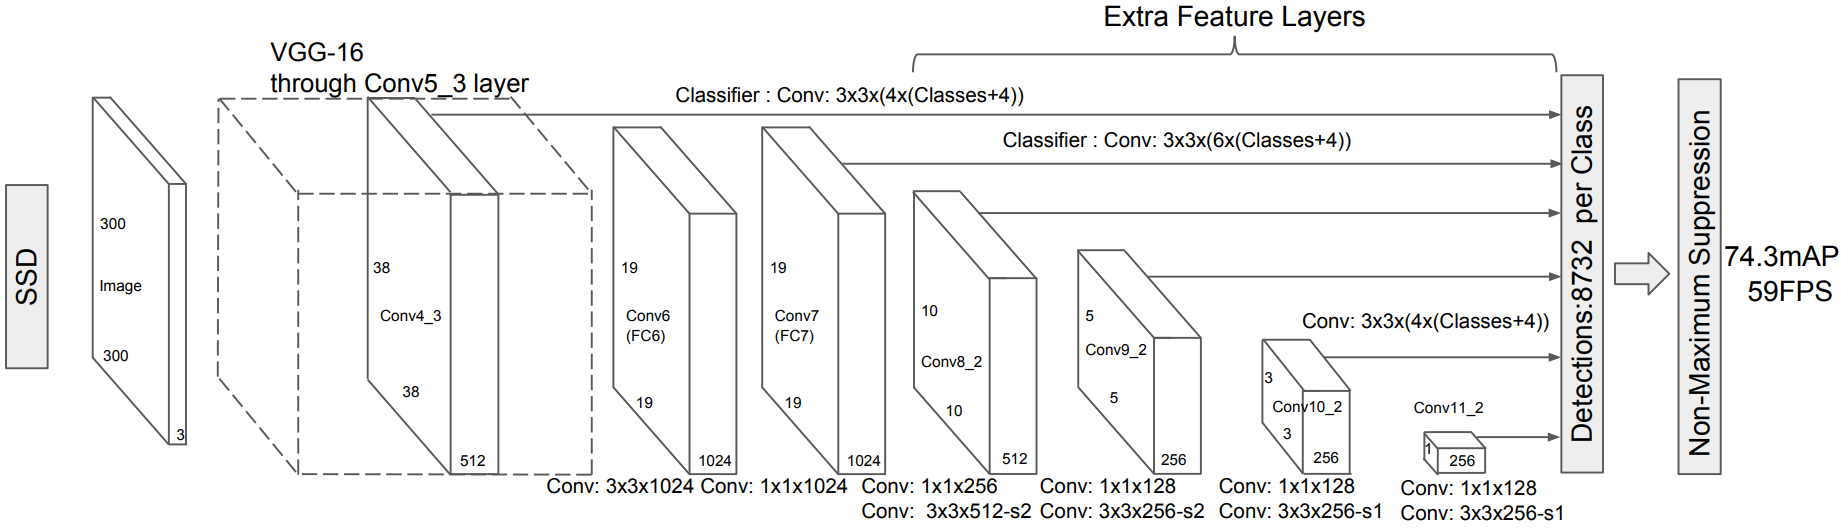
\includegraphics[width=1\textwidth]{img/algorithms/ssd-architecture.png}
    \caption{SSD architecture consists of~VGG-16 backbone followed by~additional convolutional layers. The classifiers in~extra feature layers use 3x3 convolutions for~\emph{k} (4~or~6) bounding boxes for~\emph{N} classes~+~4 offsets. Non-maximum suppression is used at~the end to handle intersecting bounding boxes (adapted from~\cite{ssd-paper}).}
    \label{ssd-architecture}
\end{figure}

SSD can be also called Single Shot MultiBox Detector because it uses multiple boxes for~localization. The original paper~\cite{ssd-paper} describes the bounding box selection as~follows. The added convolutional layers scale down so that multi-scale prediction can be done. Each of~them contributes to~the result with~its set of~detections. A~certain feature map has size \(m\)~x~\(n\) which is a number of~locations (feature map cells). A~default set of~bounding boxes is associated with~each location as~shown in~figure~\ref{ssd-multibox}.

\begin{figure}[hbt]
    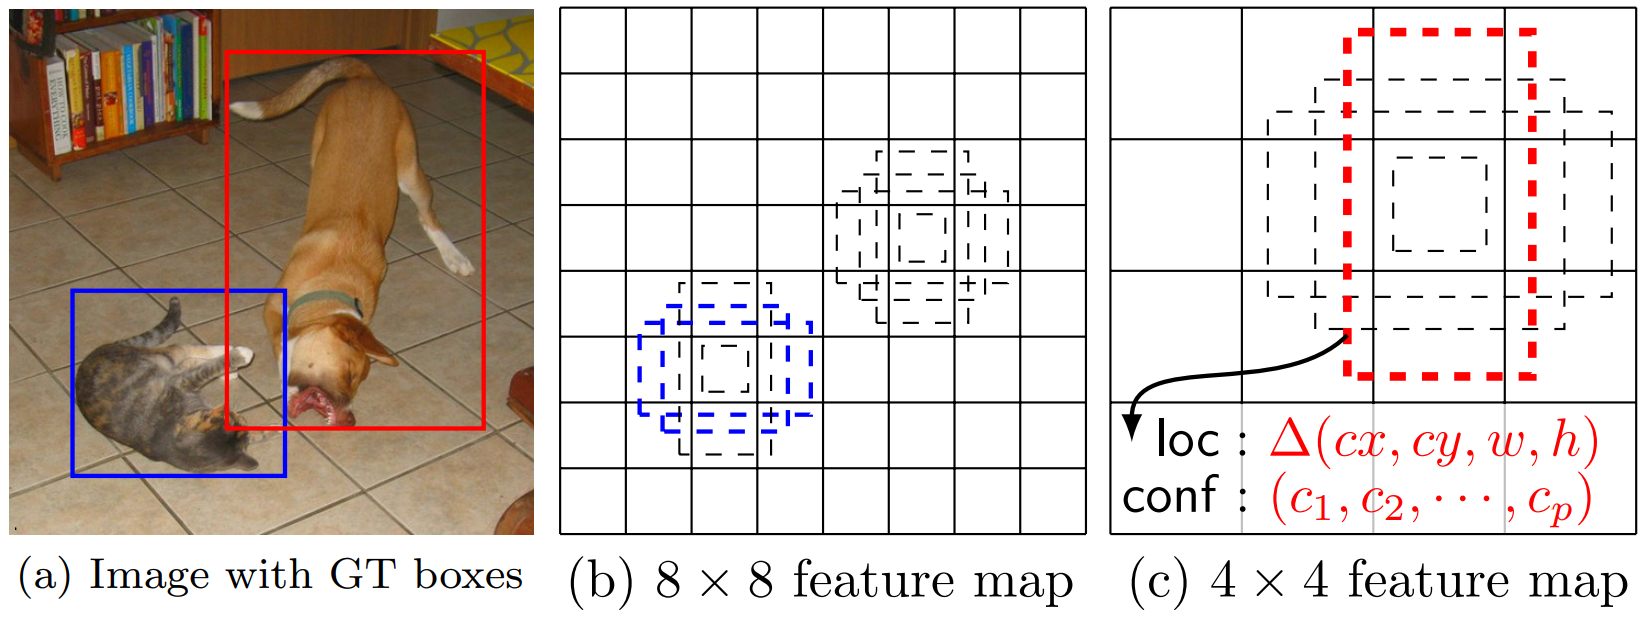
\includegraphics[width=1\textwidth]{img/algorithms/ssd-multibox.png}
    \caption{Each feature map cell has \emph{k} (usually 4~or~6) default bounding boxes. The idea is that a person, for~instance, would need a vertical box whereas a car would need a horizontal one (taken from~\cite{ssd-paper}).}    
    \label{ssd-multibox}
\end{figure}

Then we can easily get to~the~8732 detections from~figure~\ref{ssd-architecture} like this:

\begin{itemize}[topsep=0pt,itemsep=-1.5pt,partopsep=6pt]
    \item Conv4\_3: 38 x 38 x 4 = 5776
    \item Conv7: 19 x 19 x 6 = 2166
    \item Conv8\_2: 10 x 10 x 6 = 600
    \item Conv9\_2: 5 x 5 x 6 = 150
    \item Conv10\_2: 3 x 3 x 4 = 36
    \item Conv11\_2: 1 x 1 x 4 = 4
\end{itemize}

For~an image of size 300x300 is done \(5776 + 2166 + 600 + 150 + 36 + 4 = 8732\) detections. In~comparison with YOLOv1 which makes only~98 detections for~a 448x448 image, it is an extreme improvement and the main source of~the accuracy boost~\cite{ssd-paper}.

Concerning the loss function, while YOLOv1 used~5 terms based on~the sum of~squares, SSD uses only two-term loss~\ref{ssd-loss}~\cite{ssd-paper}:

\begin{equation}
  \label{ssd-loss}
  L(x, c, l, g) = \frac{1}{N}(L_{conf}(x, c) + \alpha L_{loc}(x, l, g))
\end{equation}

\(L_{conf}\) is the softmax loss function for~class prediction which takes \(x \in \{1, 0\}\) as~an indicator if the box matches the ground-truth and \emph{c} as the class confidence. \(L_{loc}\) is the Smooth L1 localization loss and \(l, g\) the predicted and ground-truth boxes respectively. \emph{N}~denotes the number of~matched bounding boxes.

Then there is the question of~how the default bounding boxes are determined. Suppose there are \emph{m} feature layers, the scale for~each layer's bounding boxes is determined by~the following equation~\ref{ssd-scale}~\cite{ssd-paper}:

\begin{equation}
  \label{ssd-scale}
  s_k = s_{min} + \frac{s_{max} - s_{min}}{m - 1} (k - 1), \hspace{0.5cm} k \in \langle1, m\rangle
\end{equation}

In~this equation \(s_{min} = 0.2\) and \(s_{max} = 0.9\), which makes the scale of~the lowest layer~0.2, the highest layer~0.9 and other layers regularly spaced. Default boxes' aspect ratios are then \(a_r \in \{1, 2, 3, \frac{1}{2}, \frac{1}{3}\}\) (excluding 3 and \(\frac{1}{3}\) when only 4 boxes are used) and a box size is computed as~\(width_k^a = s_k \sqrt{a_r}\) and \(height_k^a = \frac{s_k}{\sqrt{a_r}}\)~\cite{ssd-paper}.

The large amount of~generated bounding boxes comes with a price, though. Most of~the boxes are naturally negatives which creates an imbalance between positive and negative training samples~\cite{ssd-paper}. To~solve this issue, the hard negative mining technique is used. To~achieve more stable training and faster optimization, only the negatives with the highest confidence score are picked. In~addition to~this, to~improve the training and to~make the model more robust, data augmentation is heavily employed.

In~spite of~achieving better results than any other object detector at~the time, no further advancements or newer versions of~SSD seem to~be around. While it undoubtedly influenced many object detection architectures, SSD itself got soon dethroned as~the state-of-the-art by newer versions of~YOLO. Nevertheless, it can still be seen in~many object detection applications amongst~which the Amazon's keyboard detection~\cite{amazon-paper} can be counted.